%\documentclass[handout]{ximera}
\documentclass[nooutcomes]{ximera}

\usepackage{gensymb}
\usepackage{tabularx}
\usepackage{mdframed}
\usepackage{pdfpages}
%\usepackage{chngcntr}

\let\problem\relax
\let\endproblem\relax

\newcommand{\property}[2]{#1#2}




\newtheoremstyle{SlantTheorem}{\topsep}{\fill}%%% space between body and thm
 {\slshape}                      %%% Thm body font
 {}                              %%% Indent amount (empty = no indent)
 {\bfseries\sffamily}            %%% Thm head font
 {}                              %%% Punctuation after thm head
 {3ex}                           %%% Space after thm head
 {\thmname{#1}\thmnumber{ #2}\thmnote{ \bfseries(#3)}} %%% Thm head spec
\theoremstyle{SlantTheorem}
\newtheorem{problem}{Problem}[]

%\counterwithin*{problem}{section}



%%%%%%%%%%%%%%%%%%%%%%%%%%%%Jenny's code%%%%%%%%%%%%%%%%%%%%

%%% Solution environment
%\newenvironment{solution}{
%\ifhandout\setbox0\vbox\bgroup\else
%\begin{trivlist}\item[\hskip \labelsep\small\itshape\bfseries Solution\hspace{2ex}]
%\par\noindent\upshape\small
%\fi}
%{\ifhandout\egroup\else
%\end{trivlist}
%\fi}
%
%
%%% instructorIntro environment
%\ifhandout
%\newenvironment{instructorIntro}[1][false]%
%{%
%\def\givenatend{\boolean{#1}}\ifthenelse{\boolean{#1}}{\begin{trivlist}\item}{\setbox0\vbox\bgroup}{}
%}
%{%
%\ifthenelse{\givenatend}{\end{trivlist}}{\egroup}{}
%}
%\else
%\newenvironment{instructorIntro}[1][false]%
%{%
%  \ifthenelse{\boolean{#1}}{\begin{trivlist}\item[\hskip \labelsep\bfseries Instructor Notes:\hspace{2ex}]}
%{\begin{trivlist}\item[\hskip \labelsep\bfseries Instructor Notes:\hspace{2ex}]}
%{}
%}
%% %% line at the bottom} 
%{\end{trivlist}\par\addvspace{.5ex}\nobreak\noindent\hung} 
%\fi
%
%


\let\instructorNotes\relax
\let\endinstructorNotes\relax
%%% instructorNotes environment
\ifhandout
\newenvironment{instructorNotes}[1][false]%
{%
\def\givenatend{\boolean{#1}}\ifthenelse{\boolean{#1}}{\begin{trivlist}\item}{\setbox0\vbox\bgroup}{}
}
{%
\ifthenelse{\givenatend}{\end{trivlist}}{\egroup}{}
}
\else
\newenvironment{instructorNotes}[1][false]%
{%
  \ifthenelse{\boolean{#1}}{\begin{trivlist}\item[\hskip \labelsep\bfseries {\Large Instructor Notes: \\} \hspace{\textwidth} ]}
{\begin{trivlist}\item[\hskip \labelsep\bfseries {\Large Instructor Notes: \\} \hspace{\textwidth} ]}
{}
}
{\end{trivlist}}
\fi


%% Suggested Timing
\newcommand{\timing}[1]{{\bf Suggested Timing: \hspace{2ex}} #1}




\hypersetup{
    colorlinks=true,       % false: boxed links; true: colored links
    linkcolor=blue,          % color of internal links (change box color with linkbordercolor)
    citecolor=green,        % color of links to bibliography
    filecolor=magenta,      % color of file links
    urlcolor=cyan           % color of external links
}

\title{Congruence via Transformations}
\author{Bart Snapp and Brad Findell}

\outcome{Learning outcome goes here.}

\begin{document}
\begin{abstract}
  We think about geometric transformations.
\end{abstract}
\maketitle

\begin{teachingnote}
Supplies:  Tracing paper, long rulers for drawing these on the board.  
\end{teachingnote}

Informally, a \emph{transformation} of the plane is a ``motion,'' such
as a rotation or a stretch of the plane, that takes a figure to an
\emph{image} of that figure.  This activity explores the basic rigid
motions: translations (slides), rotations (turns), and reflections
(flips).


\begin{problem}
One of the pairs of figures below shows a translation, and the other
pair does not.  To identify which is which, draw segments between each
point and its image.  Use those segments to explain your reasoning.
\begin{image}
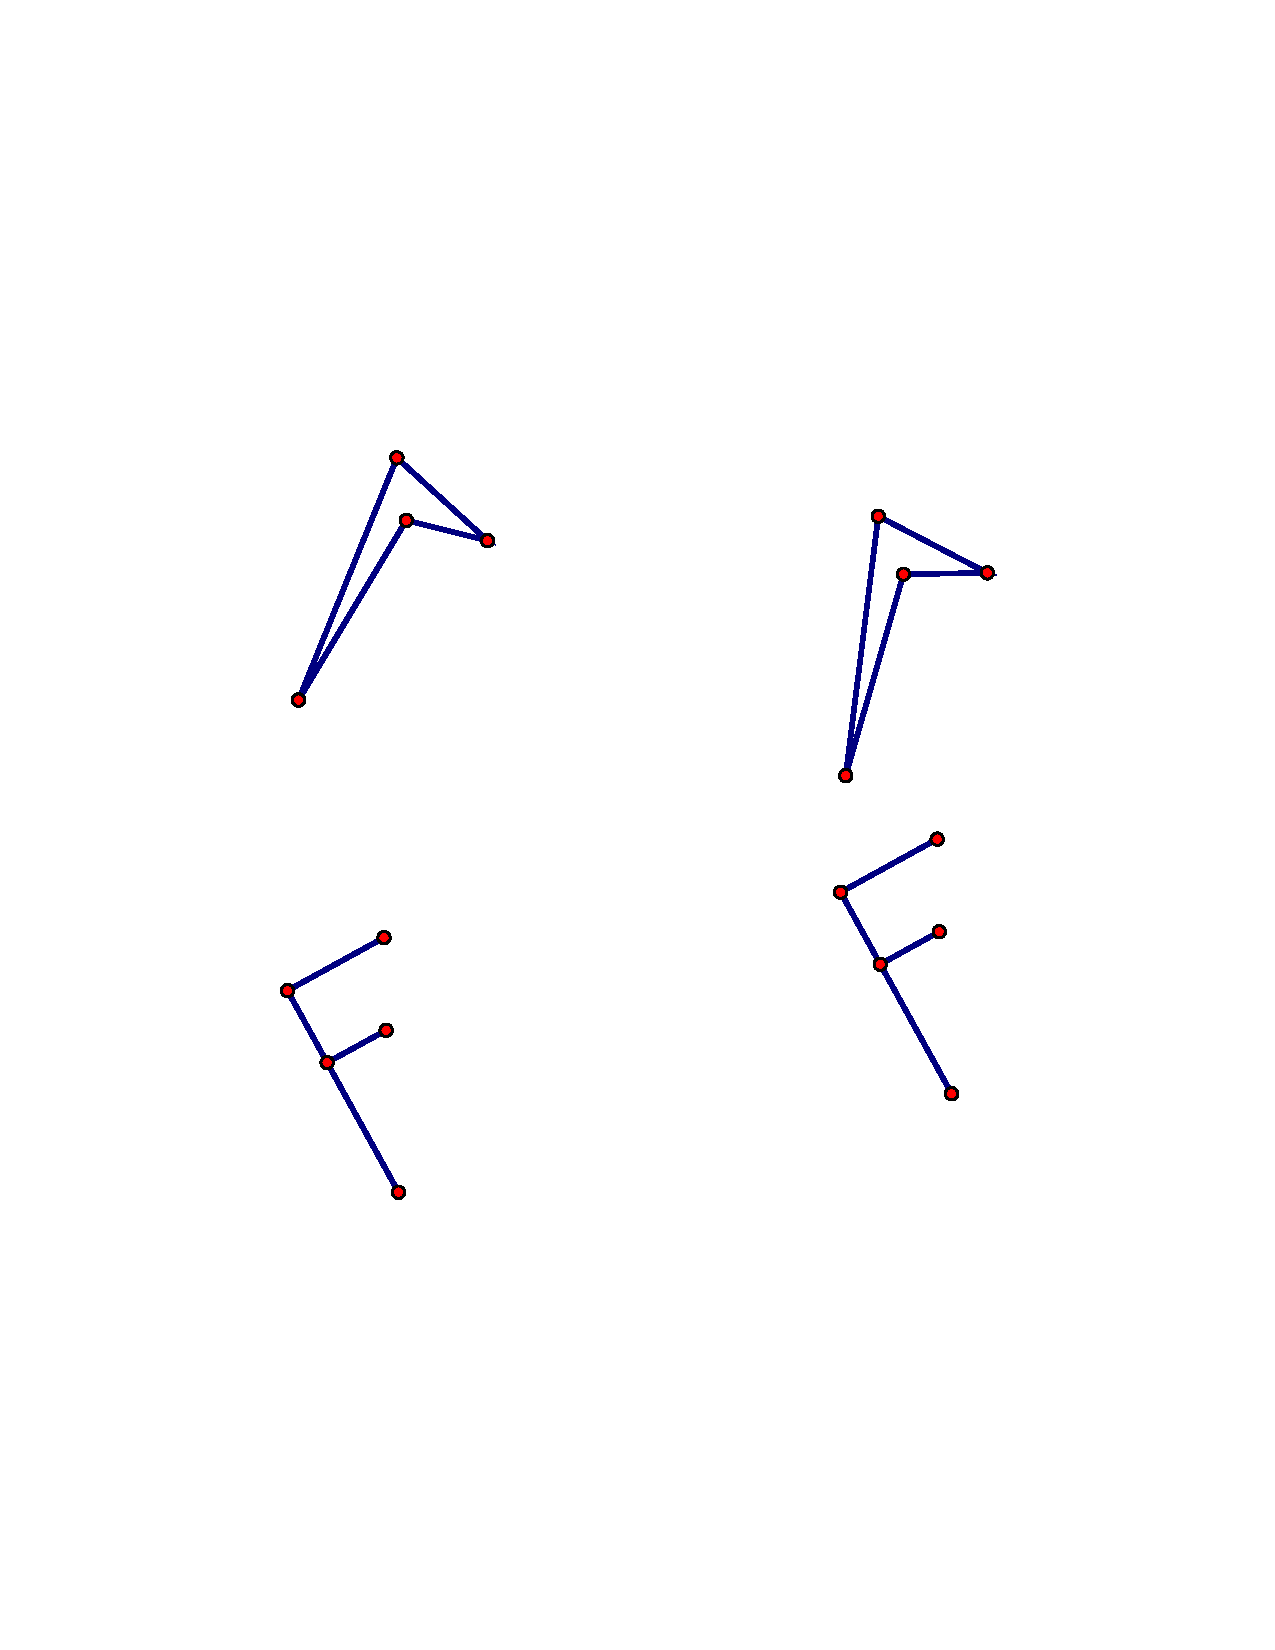
\includegraphics[scale=0.8]{translate.pdf}
\end{image}
\end{problem}

\newpage
\begin{problem}
One of the pairs of figures shows a reflection about the given line, and the other pair does not.  
\begin{enumerate}
\item Identify which pair of figures shows a reflection about the given line, and explain how you know. 
\item Find the line of reflection for the other pair of figures, and explain your reasoning.  
\begin{image}
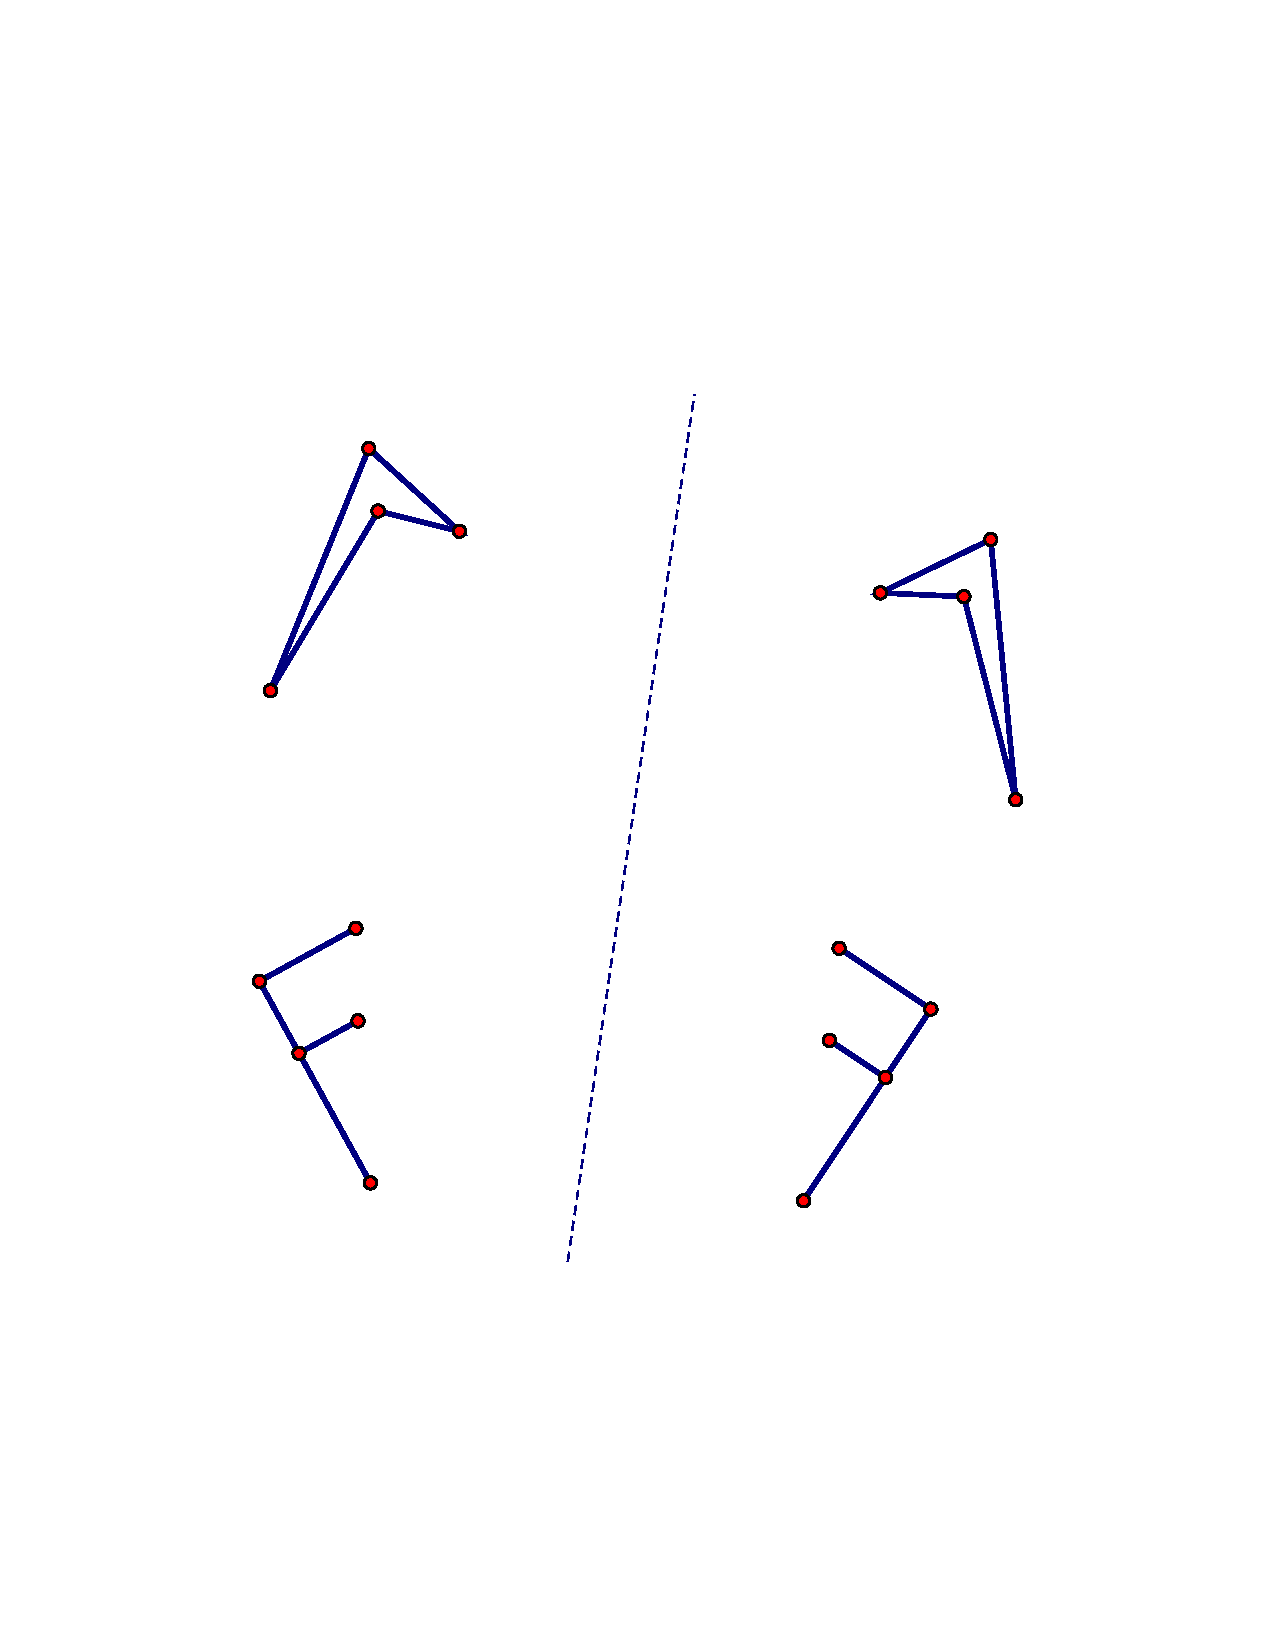
\includegraphics[scale=0.8]{reflect.pdf}
\end{image}
\end{enumerate}
\end{problem}

\newpage
\begin{problem}
One of the pairs of figures below shows a rotation about point $C$, and the other pair does not. 
\begin{enumerate}
\item Identify which pair of figures shows a rotation about $C$, and explain how you know.  
\item Find the angle of rotation.  
\item Find the center of and angle of rotation for the other pair of figures.  Explain your reasoning.  
\begin{image}
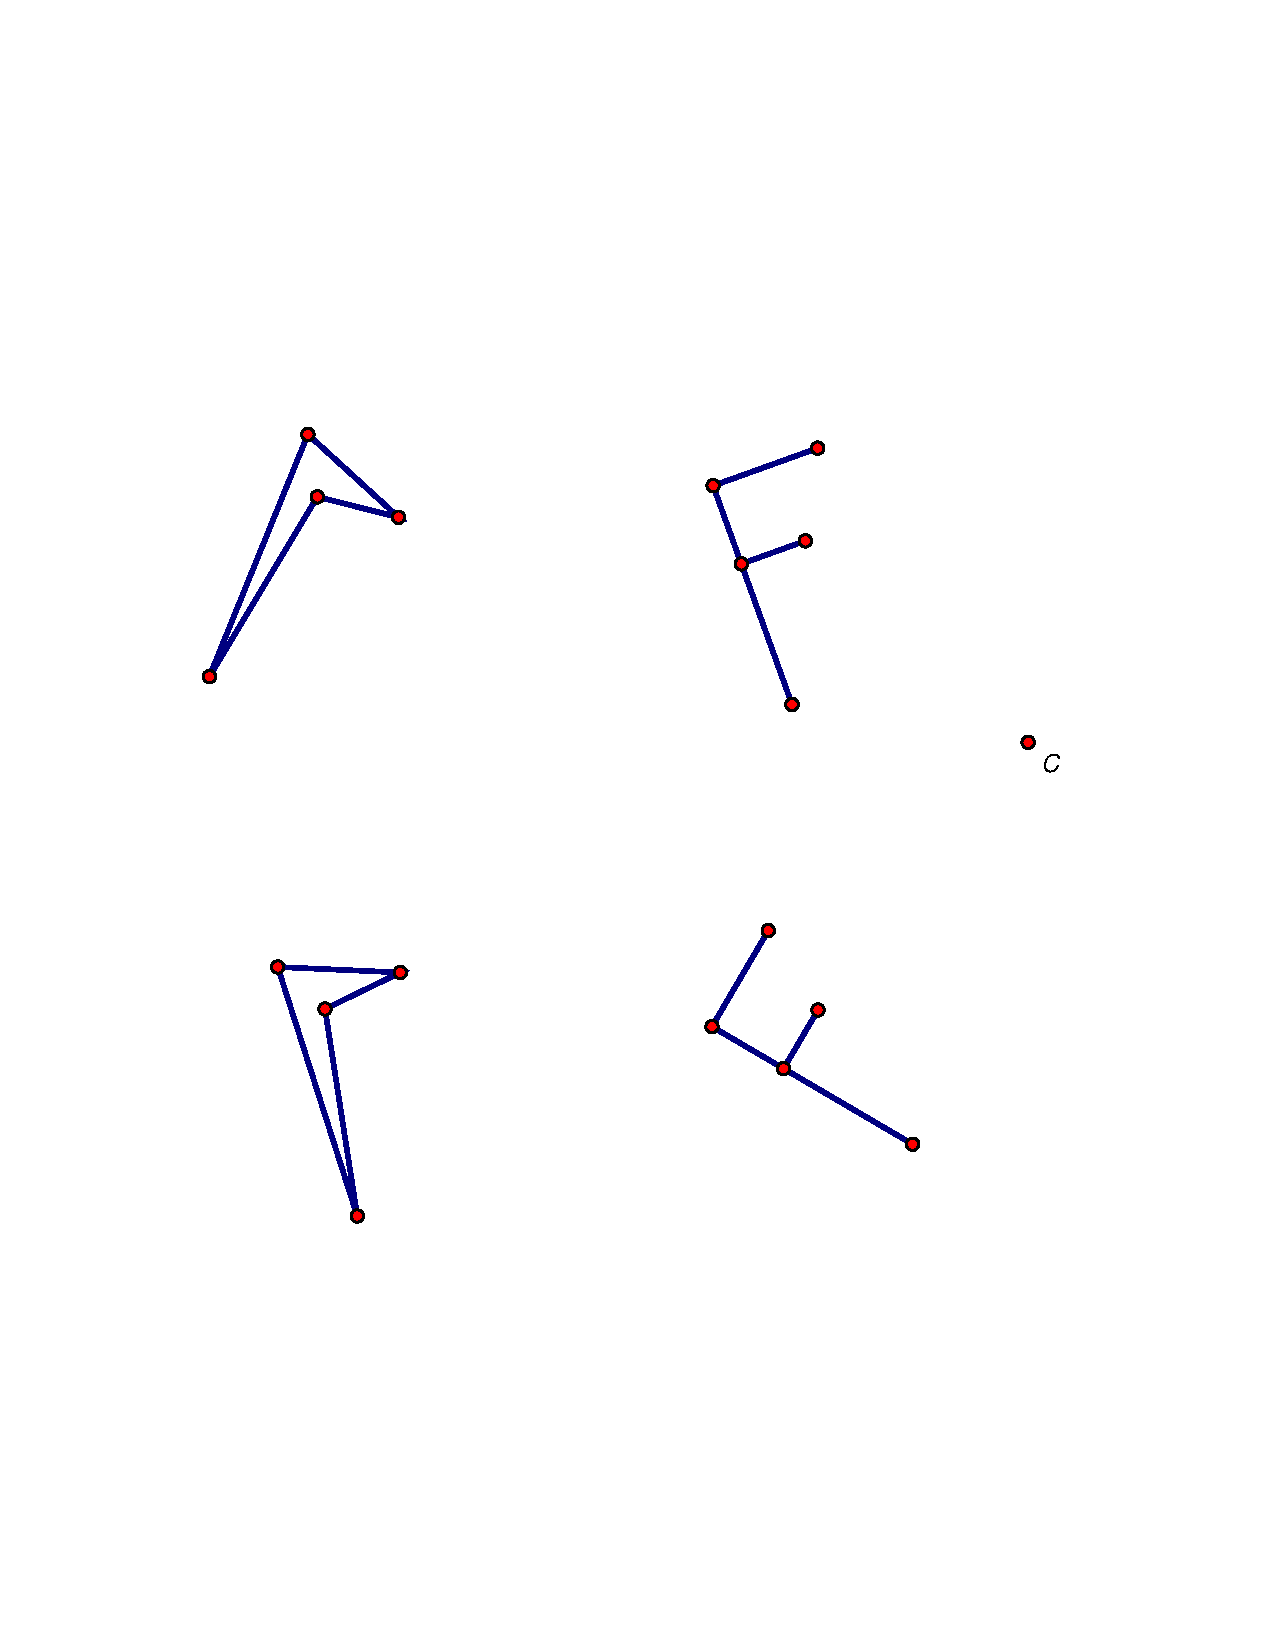
\includegraphics[scale=0.8]{../graphics/rotate.pdf}
\end{image}
\end{enumerate}
\end{problem}


\newpage
\begin{problem}
Two figures are said to be \emph{congruent} if there is a sequence of basic rigid motions that take one figure onto the other.  
\begin{enumerate}
\item Specify a sequence of two or three basic rigid motions that takes one F onto the other.  Illustrate intermediate images.  Explain your reasoning.  
\vspace{1in}
\begin{image}
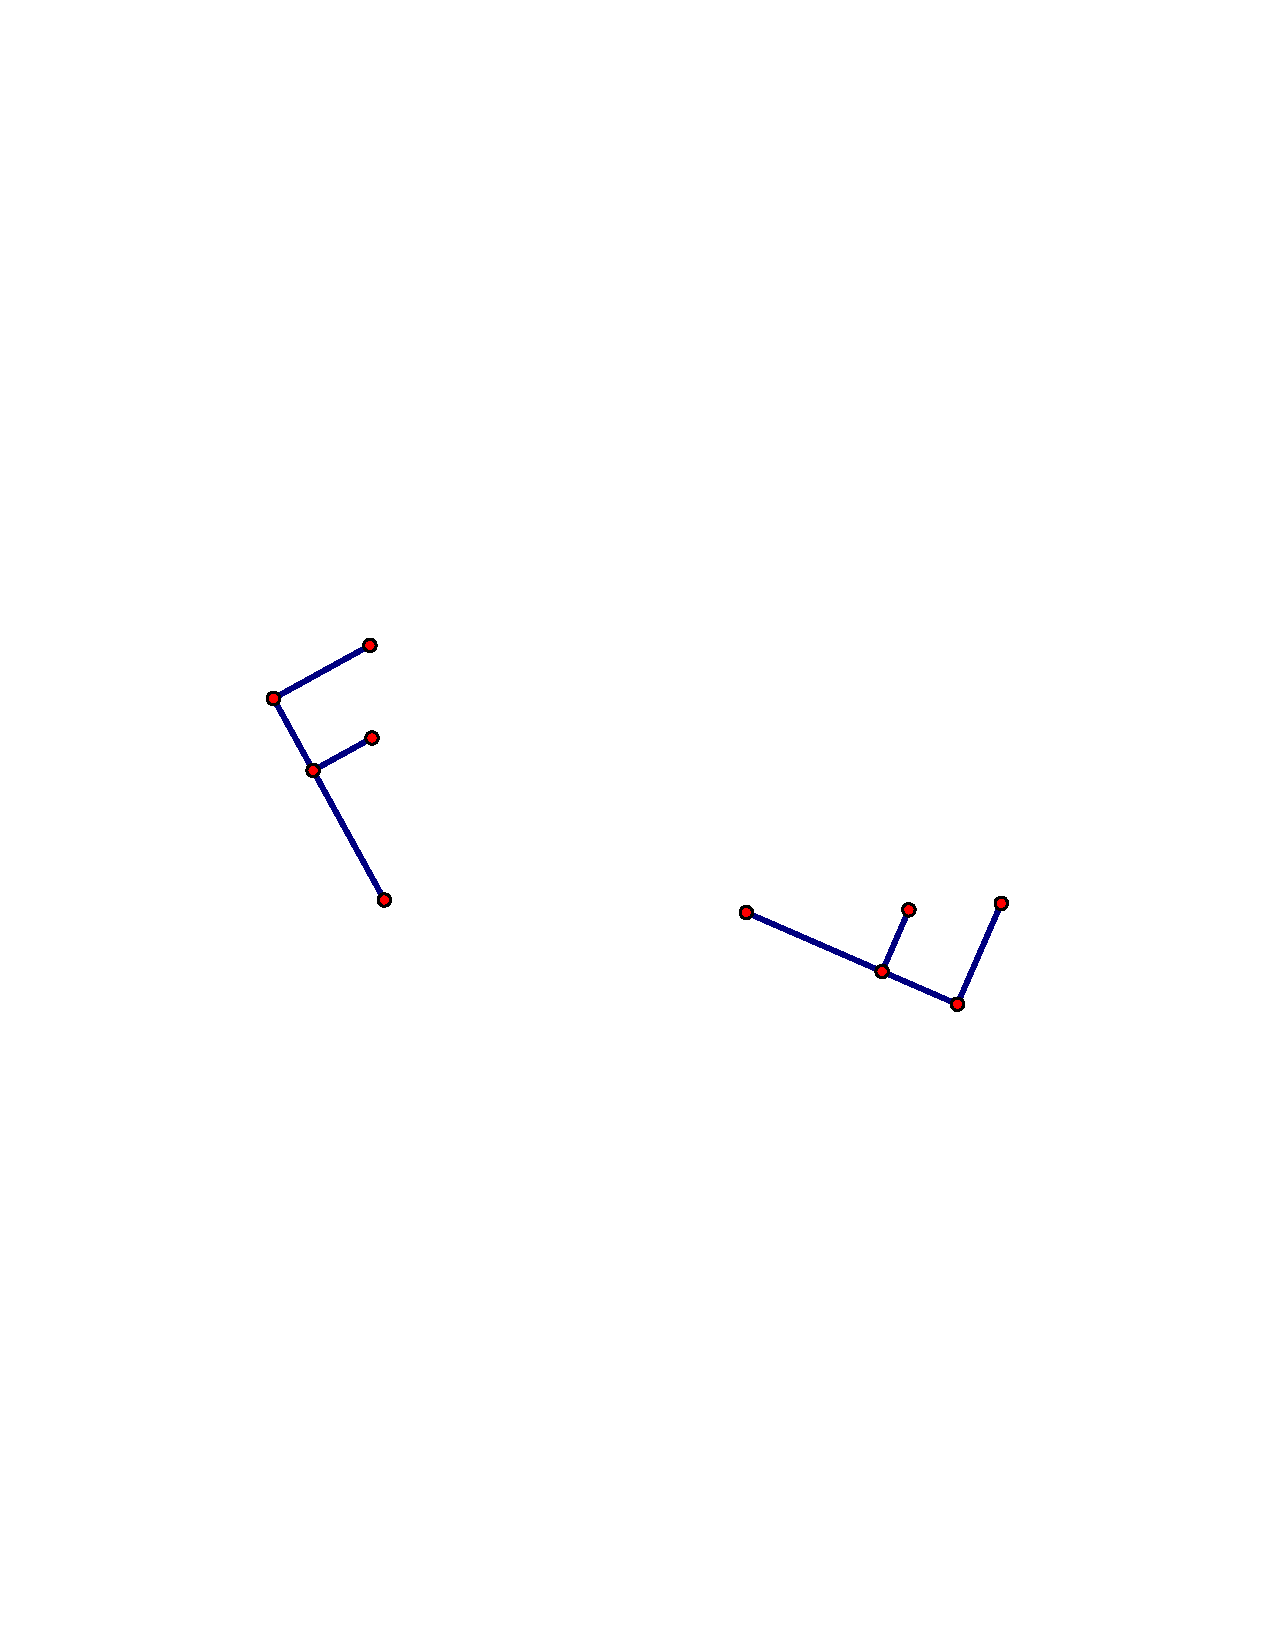
\includegraphics[scale=0.8]{../graphics/glideReflect.pdf}
\end{image}
\vspace{0.5in}
\item Explain briefly why, for this pair of figures, sequences of the following types cannot work: 
\begin{itemize}
\item a rotation followed by a rotation
\item a translation followed by a translation
\item a reflection followed by a reflection
\end{itemize}
\end{enumerate}
\end{problem}
\end{document}
